% id: 214-06
% book: 개념원리 중학 3-1 · 23 이차함수의 활용
% section: 중단원 마무리하기 STEP 1 기본 문제
% figure: crop:fig-214-06.png
% answer: ②
% answer_source: 답지
% variant_level: 0 (원본 전사)
% 이 파일은 build.mjs 가 items.json 에서 만든다. 고칠 때는 items.json 을 고친다.
\smash{\raisebox{3.5mm}{\dmkichul{개념원리 중학 3-1 214쪽 06번 · 꼭나와}}}
\noindent\begin{minipage}[t]{0.58\linewidth}\vspace{0pt}\raggedright 오른쪽 그림과 같이 이차함수 $y=-\dfrac{3}{4}x^2+3x$의 그래프의 꼭짓점을 $\pt{A}$라 하고, $x$축과의 두 교점을 각각 $\pt{O}$, $\pt{B}$라 할 때, $\triangle\pt{AOB}$의 넓이는? \cond{점~$\pt{O}$는 원점이다.}\end{minipage}\hfill\begin{minipage}[t]{0.4\linewidth}\vspace{0pt}\centering \setlength{\dmfigw}{82.5pt}\ifdim\dmfigw>\linewidth\setlength{\dmfigw}{\linewidth}\fi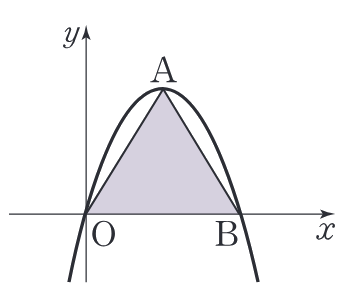
\includegraphics[width=\dmfigw]{figures/fig-214-06.png}\end{minipage}\par
\begin{choices32}{$4$}{$6$}{$8$}{$10$}{$12$}\end{choices32}
